\PassOptionsToPackage{unicode=true}{hyperref} % options for packages loaded elsewhere
\PassOptionsToPackage{hyphens}{url}
%
\documentclass[]{article}
\usepackage{lmodern}
\usepackage{amssymb,amsmath}
\usepackage{ifxetex,ifluatex}
\usepackage{fixltx2e} % provides \textsubscript
\ifnum 0\ifxetex 1\fi\ifluatex 1\fi=0 % if pdftex
  \usepackage[T1]{fontenc}
  \usepackage[utf8]{inputenc}
  \usepackage{textcomp} % provides euro and other symbols
\else % if luatex or xelatex
  \usepackage{unicode-math}
  \defaultfontfeatures{Ligatures=TeX,Scale=MatchLowercase}
\fi
% use upquote if available, for straight quotes in verbatim environments
\IfFileExists{upquote.sty}{\usepackage{upquote}}{}
% use microtype if available
\IfFileExists{microtype.sty}{%
\usepackage[]{microtype}
\UseMicrotypeSet[protrusion]{basicmath} % disable protrusion for tt fonts
}{}
\IfFileExists{parskip.sty}{%
\usepackage{parskip}
}{% else
\setlength{\parindent}{0pt}
\setlength{\parskip}{6pt plus 2pt minus 1pt}
}
\usepackage{hyperref}
\hypersetup{
            pdfborder={0 0 0},
            breaklinks=true}
\urlstyle{same}  % don't use monospace font for urls
\usepackage{longtable,booktabs}
% Fix footnotes in tables (requires footnote package)
\IfFileExists{footnote.sty}{\usepackage{footnote}\makesavenoteenv{longtable}}{}
\usepackage{graphicx,grffile}
\makeatletter
\def\maxwidth{\ifdim\Gin@nat@width>\linewidth\linewidth\else\Gin@nat@width\fi}
\def\maxheight{\ifdim\Gin@nat@height>\textheight\textheight\else\Gin@nat@height\fi}
\makeatother
% Scale images if necessary, so that they will not overflow the page
% margins by default, and it is still possible to overwrite the defaults
% using explicit options in \includegraphics[width, height, ...]{}
\setkeys{Gin}{width=\maxwidth,height=\maxheight,keepaspectratio}
\setlength{\emergencystretch}{3em}  % prevent overfull lines
\providecommand{\tightlist}{%
  \setlength{\itemsep}{0pt}\setlength{\parskip}{0pt}}
\setcounter{secnumdepth}{0}
% Redefines (sub)paragraphs to behave more like sections
\ifx\paragraph\undefined\else
\let\oldparagraph\paragraph
\renewcommand{\paragraph}[1]{\oldparagraph{#1}\mbox{}}
\fi
\ifx\subparagraph\undefined\else
\let\oldsubparagraph\subparagraph
\renewcommand{\subparagraph}[1]{\oldsubparagraph{#1}\mbox{}}
\fi

% set default figure placement to htbp
\makeatletter
\def\fps@figure{htbp}
\makeatother


\date{}

\begin{document}

\hypertarget{questions}{%
\section{Questions}\label{questions}}

\hypertarget{one}{%
\subsection{One}\label{one}}

\hypertarget{lewis-structure-of-sioh_4}{%
\subsubsection{\texorpdfstring{Lewis structure of
\(Si(OH)_4\)}{Lewis structure of Si(OH)\_4}}\label{lewis-structure-of-sioh_4}}

,\_

\hypertarget{step-1}{%
\paragraph{Step \#1}\label{step-1}}

Number of electrons = 4x6 +4x1 +1x4 = 32.

\hypertarget{step-2}{%
\paragraph{Step \#2}\label{step-2}}

After 8 electrons are assigned to each oxygen, and single bonds are
formed between each species all species have a full octet, (except for
hydrogen which has a full valence shell consisting of two electrons)

NOTE: As silica is a period two element overfilling of the octet is
possible however any additional bond formation between the oxygen and
the central silicon could only increase the formal charge and so may be
discounted.

\hypertarget{step-3}{%
\paragraph{Step \#3}\label{step-3}}

Draw structure

\begin{figure}
\centering
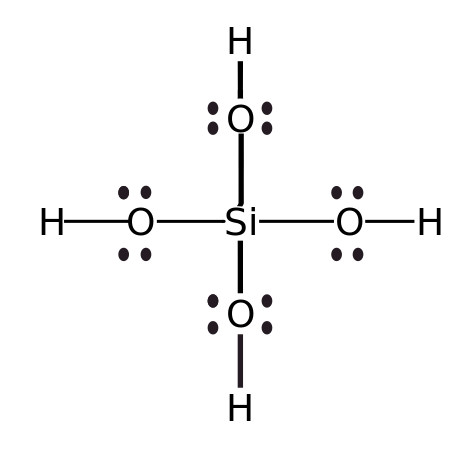
\includegraphics[width=0.5\textwidth,height=\textheight]{Images/SiliconHydroxideLewisStructure.jpg}
\caption{Silicon Hydroxide Lewis structure}
\end{figure}

\hypertarget{lewis-structure-of-aloh_4--}{%
\subsubsection{\texorpdfstring{Lewis structure of
\(Al(OH)_4 ^{-}\)}{Lewis structure of Al(OH)\_4 \^{}\{-\}}}\label{lewis-structure-of-aloh_4--}}

,\_

\hypertarget{step-1-1}{%
\paragraph{Step \#1}\label{step-1-1}}

Number of electrons = 4x6 +4x1 +1x3+1 = 32.

\hypertarget{step-2-1}{%
\paragraph{Step \#2}\label{step-2-1}}

After 8 electrons are assigned to each oxygen, and single bonds are
formed between each species all species have a full octet, (except for
hydrogen which has a full valence shell consisting of two electrons).
Again overfilling by creating more bonds will only increase the formal
charge.

\hypertarget{step-3-1}{%
\paragraph{Step \#3}\label{step-3-1}}

Draw Structure

\begin{figure}
\centering
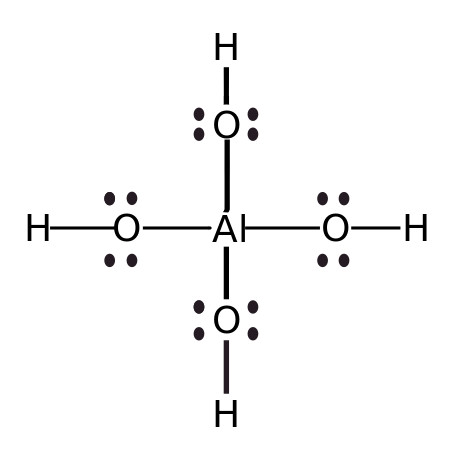
\includegraphics[width=0.5\textwidth,height=\textheight]{Images/AluminiumHydroxideIonLewisStructure.jpg}
\caption{Aluminium Hydroxide Ion Lewis structure}
\end{figure}

\hypertarget{lewis-structure-of-aloh_3}{%
\subsubsection{\texorpdfstring{Lewis Structure of
\(Al(OH)_3\)}{Lewis Structure of Al(OH)\_3}}\label{lewis-structure-of-aloh_3}}

,\_

\hypertarget{step-1-2}{%
\paragraph{Step \#1}\label{step-1-2}}

Number of electrons = 3x6 +3x1 +1x3= 32

\hypertarget{step-2-2}{%
\paragraph{Step \#2}\label{step-2-2}}

After 8 electrons are assigned to each oxygen, and single bonds are
formed between each species all species have a full octet, (except for
hydrogen which has a full valence shell consisting of two electrons).
Again overfilling by creating more bonds will only increase the formal
charge.

\hypertarget{step-3-2}{%
\paragraph{Step \#3}\label{step-3-2}}

Draw Structure

\begin{figure}
\centering
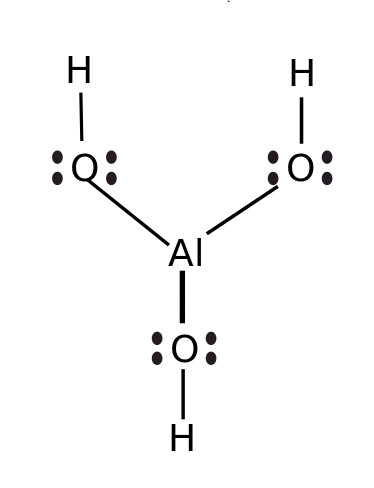
\includegraphics[width=0.5\textwidth,height=\textheight]{Images/AluminiumHydroxideLewisStructure.jpg}
\caption{Aluminium Hydroxide Ion Lewis structure}
\end{figure}

\hypertarget{two}{%
\subsection{Two}\label{two}}

\hypertarget{i}{%
\subsubsection{(i)}\label{i}}

\hypertarget{step-1-3}{%
\paragraph{Step \#1}\label{step-1-3}}

Moles of EDTA added to EDTA standard

\(= \frac{0.914g}{372.24g.mol^{-1}}\)
\(= 2.4554 \quad x \quad 10^{-3}mol\)

\hypertarget{step-2-3}{%
\paragraph{Step \#2}\label{step-2-3}}

Average Titrant volume \(= 0.5x ((4.57-0.04)+(5.13-0.10))ml= 4.78ml\)

\hypertarget{step-3-3}{%
\paragraph{Step \#3}\label{step-3-3}}

Moles of EDTA in Titrant

\(= 2.4554 \quad x \quad 10^{-3}mol \quad x \quad \frac{4.78ml}{250ml}\)

\(= 4.6947 \quad x \quad 10^{-5}mol\)

\hypertarget{ii}{%
\subsubsection{(ii)}\label{ii}}

\hypertarget{step-1-4}{%
\paragraph{Step \#1}\label{step-1-4}}

At equivalence point of the titration all of the EDTA has reacted with
calcium at the ratio of 1 mol EDTA: 1 mol calcium ions.

Hence If \(= 4.6947 \quad x \quad 10^{-5}mol\) of calcium where added
then \(= 4.6947 \quad x \quad 10^{-5}mol\) of calcium ions where used up
form the titrand.

\hypertarget{step-2-4}{%
\paragraph{Step \#2}\label{step-2-4}}

As the titrand contained only 25ml of the original calcium chloride
zeolite solution, It can be interpolated that
\(3 \quad x\quad 4.6947 \quad x \quad 10^{-5}mol= 1.4084 \quad x \quad 10^{-4}\)\\
of calcium ions would have been used up from the entire solution.

\hypertarget{iii}{%
\subsubsection{(iii)}\label{iii}}

\hypertarget{step-1-5}{%
\paragraph{Step \#1}\label{step-1-5}}

Moles of Calcium chloride present in the original solution.

\(\quad = \frac{0.196g}{219.08g.mol^{-1}}\)

\(\quad = 8.9465 \quad x \quad 10{-4}\)

\hypertarget{step-3-4}{%
\paragraph{Step \#3}\label{step-3-4}}

Moles of Calcium ions left in the original solution

\(\quad = 8.9465 \quad x \quad 10^{-4}mol - 1.4084 \quad x \quad 10^{-4}mol\)

\(\quad 7.5381 x \quad 10^{-4}mol\)

\hypertarget{iv}{%
\subsubsection{(iv)}\label{iv}}

Grams of Calcium chloride left in original solution.
\(\quad = 7.5381 x \quad 10^{-4}mol \quad x \quad 40.08g.mol^{-1}\)
\(\quad = 3.0213 \quad x \quad 10^{-2}g\)

\hypertarget{v}{%
\subsubsection{(v)}\label{v}}

\hypertarget{step-1-6}{%
\paragraph{Step \#1}\label{step-1-6}}

The amount of calcium ions taken up by the zeolite is equivalent to the
amount fo calcium ions remaining in solution, as any calcium ions not
bound would have been removed during the EDTA titration.

Hence there are \(7.5381 \quad x \quad 10^{-4}mol\) of Calcium ions
bound by the zeolite.

\hypertarget{vi}{%
\subsubsection{(vi)}\label{vi}}

\hypertarget{step-1-7}{%
\paragraph{Step \#1}\label{step-1-7}}

Grams of Calcium ions taken up per gram of Zeolite

\(\quad = \frac{3.0213 \quad x \quad 10^{-2}g}{0.104g}\)

\(\quad = 0.29051 (g/g)\)

\hypertarget{three}{%
\subsection{Three}\label{three}}

This implies that zeolites may be very useful as detergents as they are
capable of sequestering/removing relatively large quantities of
dissolved ions from solution. (removing these ions will prevent them
from resettling on whatever item is being cleaned, and increase the
overall ability of the detergent to dissolve and remove unwanted
deposits from the item being cleaned.)

\hypertarget{five}{%
\subsection{Five}\label{five}}

four acid sites are accosted with the EDTA. (one for each of the
terminal carboxylic acid groups)

\hypertarget{six.}{%
\subsection{Six.}\label{six.}}

Yes. Sulphuric acid has the same activity of any normal acid catalyst,
providing a ready source and sink for \(H^{+}\) ions, facilitating the
internal structural changes necessary for ester formation.

\hypertarget{seven}{%
\subsection{Seven}\label{seven}}

Pentyl ethanol is used:

\begin{enumerate}
\def\labelenumi{\arabic{enumi}.}
\item
  as a flavourant in many foods.
\item
  As a solvent in paints.
\end{enumerate}

\hypertarget{eight}{%
\subsection{Eight}\label{eight}}

Zeolite is micro-porous, that is within its 3D chemical structure there
is a regular arrangement of regular sized gaps/holes/pores,through which
other molecules, if sufficiently small could pass through. molecules
which are too large however, (such as molecules with a diameter greater
than X in the figure below) can. Such molecules suffer size exclusion,
as although they may have the correct chemical properties to react with
binding sites on the interior, they are physically prevented from
reaching these sites, as the are too large, and so cannot bind.

\begin{figure}
\centering
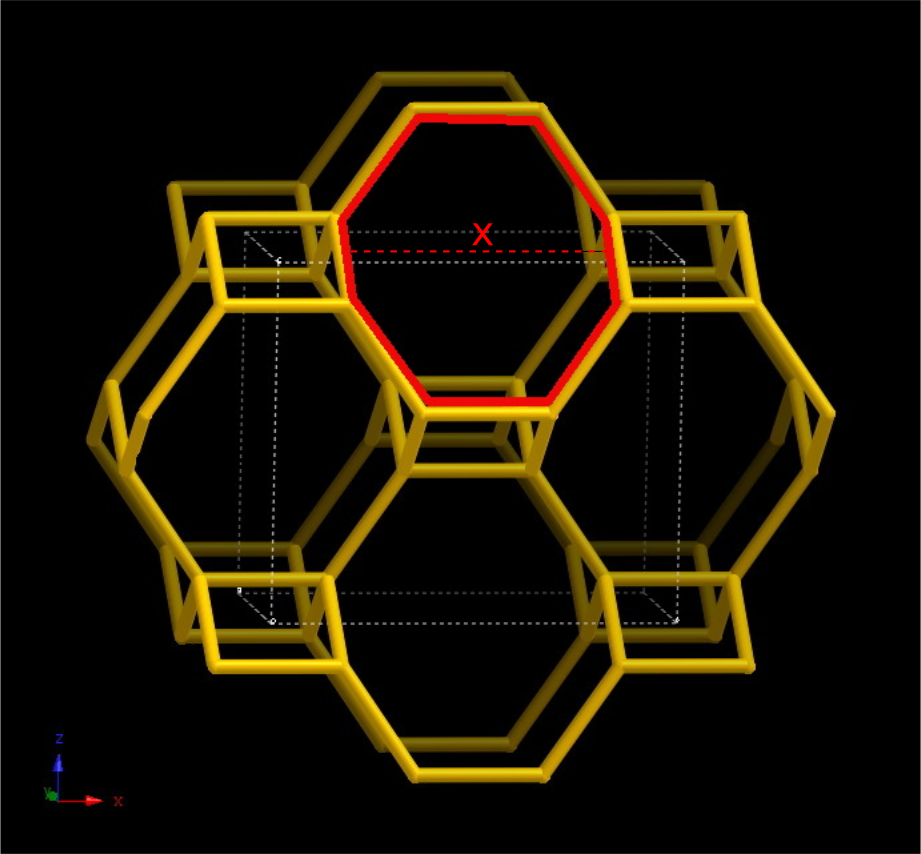
\includegraphics[width=0.5\textwidth,height=\textheight]{Images/ZeoliteStructure2.jpg}
\caption{Zeolite Structure}
\end{figure}

\hypertarget{aim}{%
\section{Aim}\label{aim}}

Two different experiments where performed with different aims.

The aim of experiment A was to determine the Ability of Zeolite to bind
Calcium ions from solution. Both to determine how effective Zeolite
could be as a cleaning/filtering agent to remove calcium impurities, and
to approximate how much zeolite (by mass) would be necessary to remove
calcium from a contaminated solution.

The aim of experiment B was to determine Zeolite ability to act as a
Acid catalyst (in esterification.)

\hypertarget{introduction}{%
\section{Introduction}\label{introduction}}

Zeolites Are complex three dimensional molecules formed from the
condensation of \$Si(OH)\emph{\{4\} \$} and \(Ai(OH)^{-}_{4}\) monomers.
These monomers take a variety of forms including cages, chains, channels
and sheets(Cejka, 2007). When these monomers bond together three
dimensional structure/nets can be formed.The most striking feature of
the complexes formed is the regularly sized and evenly space pores which
are most commonly composed of six or eight bonded tetrahedral units,
forming hexagonal or octagonal openings in the molecule respectively.
(See the figure below). This regular arrangement has many potentially
important chemical applications. One such application is the ability of
Zeolites to act as molecular sponges/ filters soaking up particles of
the correct size to fit through the microspores which binding to the
interior of the molecule via a process of cation exchange. this process
can be effect in removing cation contaminants from solution.(Motsi et Al
2009). Furthermore Zeolites can also act as effective inorganic acid
catalyst, (provided they contain appropriate ratios of aluminium to
silicon subunits). these catalyst have been demonstrated to be more
effective that simple lewis or bronsted acids in catalysing important
organic synthesis pathways such as the etherification of glycerol.(Aula
et Al 2017) Such catalyst have the added advantage that, as the catalyst
is solid state, removal and reuse if far simpler and less energetically
expensive than a conventional acid catalyst.

\hypertarget{section}{%
\subsection{}\label{section}}

\begin{figure}
\centering
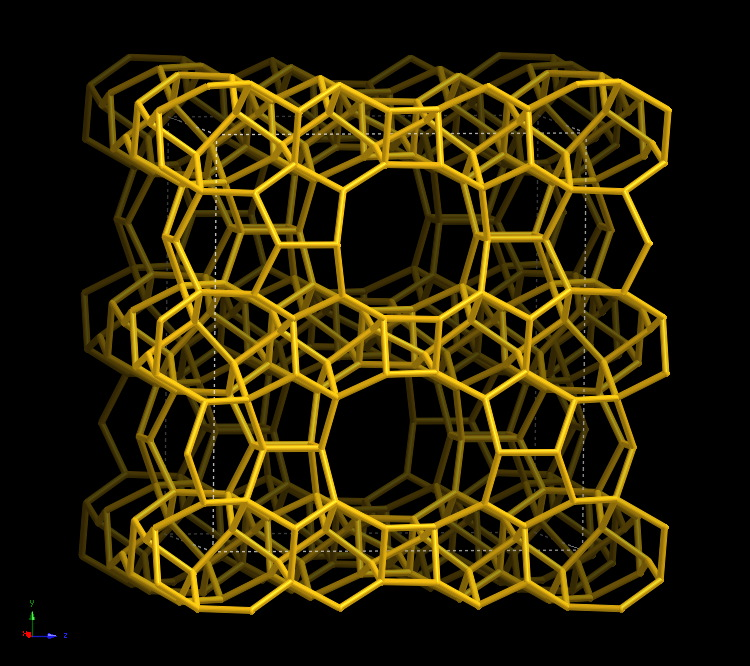
\includegraphics[width=0.5\textwidth,height=\textheight]{Images/ZeoliteStructure.jpg}
\caption{Zeolite Structure}
\end{figure}

\hypertarget{results-and-discussion.}{%
\section{Results and discussion.}\label{results-and-discussion.}}

A was them mas ratio of grams of calcium taken up per gram of
zeolite,calculated as \(\quad = 0.291 (g/g)\). This importance of this
figure

\hypertarget{material-and-methods}{%
\section{Material and methods}\label{material-and-methods}}

\hypertarget{experiment-a.}{%
\subsection{Experiment A.}\label{experiment-a.}}

\hypertarget{preparation-of-standards}{%
\subsubsection{Preparation of
standards}\label{preparation-of-standards}}

In the first main experiment two standard solutions where prepared, A
\(\approx\) 0.01M \(CaCl_2.6H_2O\) solution and a \(\approx\) 0.01M EDTA
disodium salt solution. (The exact masses of \(CaCl_2.6H_2O\) and EDTA
disodium salt can be referenced in the Data appendices.). In each case
deionised water was used to make up the solution to prevent unwanted
cations or other contaminants from affecting the experiment result.

\hypertarget{preparation-of-analyte.}{%
\subsubsection{Preparation of Analyte.}\label{preparation-of-analyte.}}

\(\approx\) of zeolite was added to 75ml of the \(CaCl_2.6H_2O\)
standard solution, and mixed by means of a magnetic stirrer bar for a
period of approximately five minutes. Subsequently the zeolite was
removed by filtration through a gravity filter. And samples of solution
where taken to serve as the analyte for titration against the EDTA
di-sodium salt standard solution.

\hypertarget{titration}{%
\subsubsection{Titration}\label{titration}}

titration was performed in triplicate however one titration had to be
discounted because of inaccuracies in identification of the endpoint.
(Eriochrome black T was used as the indicator). the remaining two
titration values where averaged.

\hypertarget{experiment-b}{%
\subsection{Experiment B}\label{experiment-b}}

\hypertarget{preparation-of-initial-solutions.}{%
\subsubsection{Preparation of initial
solutions.}\label{preparation-of-initial-solutions.}}

2 solutions where prepared, solution one containing:

\textbar{}----------------------------------\textbar{} \textbar{}
Glacial Acetic acid \textbar{} 15ml \textbar{} \textbar{}
\textbar{}----------------------------------\textbar{} \textbar{}
1-pentanol \textbar{} 15ml \textbar{} \textbar{}
\textbar{}----------------------------------\textbar{} \textbar{}
sulphuric acid \textbar{} 1ml \textbar{} \textbar{}

And solution two containing:

\textbar{}----------------------------------\textbar{} \textbar{}
Glacial Acetic acid \textbar{} 15ml \textbar{} \textbar{}
\textbar{}----------------------------------\textbar{} \textbar{}
1-pentanol \textbar{} 15ml \textbar{} \textbar{}
\textbar{}----------------------------------\textbar{} \textbar{}
Zeolite \textbar{} 2g \textbar{} \textbar{}

\hypertarget{synthesis}{%
\subsection{Synthesis}\label{synthesis}}

both solutions where then boiled under reflux for approximately an hour.

\hypertarget{work-up}{%
\subsubsection{Work up}\label{work-up}}

after cooling the solutions where rinsed several times with water to
remove any remaining acid or alcohol impurities.

\hypertarget{data-appendices}{%
\section{Data Appendices}\label{data-appendices}}

\hypertarget{experiment-a.-1}{%
\subsection{Experiment A.}\label{experiment-a.-1}}

\hypertarget{materials-used}{%
\subsubsection{Materials used}\label{materials-used}}

\begin{longtable}[]{@{}l@{}}
\toprule
Materials used in preparation\tabularnewline
\midrule
\endhead
Weight of hydrated Calcium Chloride used in Solution 1\tabularnewline
--------------------------------------------------------\tabularnewline
Weight of EDTA disodium salt use in Solution 2\tabularnewline
--------------------------------------------------------\tabularnewline
Weight of Zeolite added to Solution 1\tabularnewline
\bottomrule
\end{longtable}

\hypertarget{titration-table}{%
\subsubsection{Titration Table}\label{titration-table}}

\begin{longtable}[]{@{}l@{}}
\toprule
Titration of solution 2, (titrant) into solution 1
(Analyte)\tabularnewline
\midrule
\endhead
Titration number\tabularnewline
------------------\tabularnewline
\#1\tabularnewline
\#2\tabularnewline
\bottomrule
\end{longtable}

\hypertarget{experiment-b.}{%
\subsection{Experiment B.}\label{experiment-b.}}

\hypertarget{description-of-product.}{%
\subsubsection{Description of product.}\label{description-of-product.}}

\begin{longtable}[]{@{}lll@{}}
\toprule
\begin{minipage}[b]{0.35\columnwidth}\raggedright
\strut
\end{minipage} & \begin{minipage}[b]{0.20\columnwidth}\raggedright
Density\strut
\end{minipage} & \begin{minipage}[b]{0.36\columnwidth}\raggedright
Smell\strut
\end{minipage}\tabularnewline
\midrule
\endhead
\begin{minipage}[t]{0.35\columnwidth}\raggedright
pentyl ethanoate prepared using sulphuric acid catalyst.\strut
\end{minipage} & \begin{minipage}[t]{0.20\columnwidth}\raggedright
Lighter than (deionised) water\strut
\end{minipage} & \begin{minipage}[t]{0.36\columnwidth}\raggedright
Fruity aroma, reminiscent of banana,intoxicating fumes.\strut
\end{minipage}\tabularnewline
\begin{minipage}[t]{0.35\columnwidth}\raggedright
pentyl ethanoate prepared using Zeolite acid catalyst.\strut
\end{minipage} & \begin{minipage}[t]{0.20\columnwidth}\raggedright
Lighter than (deionised) water\strut
\end{minipage} & \begin{minipage}[t]{0.36\columnwidth}\raggedright
Intense fruity aroma, reminiscent of banana\strut
\end{minipage}\tabularnewline
\begin{minipage}[t]{0.35\columnwidth}\raggedright
---------------------------------------------------------\strut
\end{minipage} & \begin{minipage}[t]{0.20\columnwidth}\raggedright
--------------------------------\strut
\end{minipage} & \begin{minipage}[t]{0.36\columnwidth}\raggedright
----------------------------------------------------------\strut
\end{minipage}\tabularnewline
\bottomrule
\end{longtable}

\#References In-text: (Cejka, 2007)

Cejka, J. (2007). Introduction to zeolite molecular sieves. Amsterdam:
Elsevier, p.15

T. Motsi, N.A. Rowson, M.J.H.Simmons, Adsorption of heavy metals from
acid mine drainage by atural zeolite, International Journal of Mineral
Processing, Volume 92, Issues 1--2, 2009, Pages 42-48,ISSN 0301-7516,

Aula M. Veiga, Alexandre C.L. Gomes, Cláudia O. Veloso, Cristiane A.
Henriques, Acid zeolites for glycerol etherification with ethyl alcohol:
Catalytic activity and catalyst properties, Applied Catalysis A:
General, Volume 548, 2017, Pages 2-15,ISSN 0926-860X,

\end{document}
